% This LaTeX was auto-generated from MATLAB code.
% To make changes, update the MATLAB code and export to LaTeX again.

\documentclass{article}

\usepackage[utf8]{inputenc}
\usepackage[T1]{fontenc}
\usepackage{lmodern}
\usepackage{graphicx}
\usepackage{color}
\usepackage{hyperref}
\usepackage{amsmath}
\usepackage{amsfonts}
\usepackage{epstopdf}
\usepackage[table]{xcolor}
\usepackage{matlab}

\sloppy
\epstopdfsetup{outdir=./}
\graphicspath{ {./HW8_code_images/} }

\matlabhastoc

\matlabmultipletitles

\begin{document}
	
\maketitle
\thispagestyle{empty}
\pagebreak
\matlabtableofcontents{Table of Contents}

	

\begin{par}
\begin{flushleft}
Through this homework assignment we will download CIFAR-10 dataset and try to train an AlexNet-like neural network to classify the images in the dataset.
\end{flushleft}
\end{par}

\begin{matlabcode}
% to load last saved variables to worksapce of Matlab
load('HW8_code_workspace.mat')
\end{matlabcode}

\pagebreak

\label{T_5E2A80B1}
\matlabtitle{0. CIFAR-10 Dataset}

\begin{par}
\begin{flushleft}
CIFAR-10 dataset is a collection of 60,000 labeled images (50,000 for training and 10.000 for testing) of 10 classes which were collected by Alex Krizhevsky, Vinod Nair, and Geoffrey Hinton. In this section we are going to download, unzip and load it into \textit{Matlab}.
\end{flushleft}
\end{par}

\label{H_3EEF28B8}
\matlabheading{0.1 Downloading CIFAR-10 Dataset}

\begin{par}
\begin{flushleft}
The code below will check if there exist the dataset and if not, it will download both the train and test set of CIFAR-10.
\end{flushleft}
\end{par}

\begin{matlabcode}
clc; clear; close all;

if ~exist('cifar-10-batches-mat','dir')
    cifar10Dataset = 'cifar-10-matlab';
    disp('Downloading 174MB CIFAR-10 dataset...');   
    websave([cifar10Dataset,'.tar.gz'],...
        ['https://www.cs.toronto.edu/~kriz/',cifar10Dataset,'.tar.gz']);
    gunzip([cifar10Dataset,'.tar.gz'])
    delete([cifar10Dataset,'.tar.gz'])
    untar([cifar10Dataset,'.tar'])
    delete([cifar10Dataset,'.tar'])
else
    disp('CIFAR-10 dataset already downloaded.')
end
\end{matlabcode}
\begin{matlaboutput}
CIFAR-10 dataset already downloaded.
\end{matlaboutput}


\label{H_3655A561}
\matlabheading{0.2 Splitting CIFAR-10 into Folders by Their Labels}

\begin{par}
\begin{flushleft}
After downloading the dataset, we need to put every single image in a folder which has the name equal to the image's label. Doing that will make it easier for us to use built-in Matlab function to load the dataset into Matlab workspace.
\end{flushleft}
\end{par}

\begin{matlabcode}
if ~exist('cifar10Train','dir')
    disp('Saving the Images in folders. This might take some time...');    
    saveCIFAR10AsFolderOfImages('cifar-10-batches-mat', pwd, true);
else
    disp('CIFAR-10 dataset already foldered!')
end
\end{matlabcode}
\begin{matlaboutput}
CIFAR-10 dataset already foldered!
\end{matlaboutput}


\label{H_B6C31EEF}
\matlabheading{0.3 Loading Training Images into \textit{Matlab}}

\begin{par}
\begin{flushleft}
Using built-in \textit{\textbf{imageDatastore}} of \textit{Matlab }will help us to import data in batches, so they could be fit into memory easily.
\end{flushleft}
\end{par}

\begin{matlabcode}
categories = {'airplane', 'truck', 'horse',...
              'deer','dog','frog', ...
              'cat', 'ship', 'bird', 'automobile'};

rootFolder = 'cifar10Train';
imds = imageDatastore(fullfile(rootFolder, categories), ...
    'LabelSource', 'foldernames');
clear rootFolder

disp(countEachLabel(imds));
\end{matlabcode}
\begin{matlaboutput}
      Label       Count
    __________    _____

    airplane      5000 
    automobile    5000 
    bird          5000 
    cat           5000 
    deer          5000 
    dog           5000 
    frog          5000 
    horse         5000 
    ship          5000 
    truck         5000 
\end{matlaboutput}


\label{H_87B337A2}
\matlabheading{0.4 Plot One Random Sample of Each Class}

\begin{par}
\begin{flushleft}
We plot one sample of every class in the training dataset.
\end{flushleft}
\end{par}

\begin{matlabcode}
rand_nums = randi(size(imds.Files, 1)/10) + [0:5000:45000];

figure('Position', [100, 100, 1000, 1000]);
for i = 1:10
    subplottight(3,4,i);
    imshow(imread(imds.Files{rand_nums(i)}), 'border', 'tight');
    title(char(imds.Labels(rand_nums(i))));
    hold on;
end
hold off
\end{matlabcode}
\begin{center}
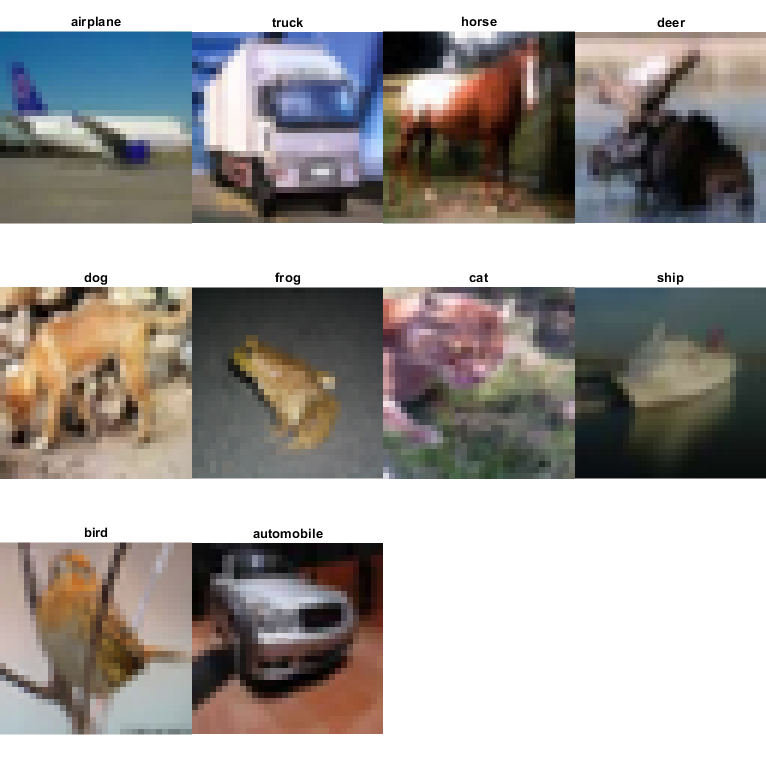
\includegraphics[scale=0.5]{figure_0.png}
\end{center}

\clearpage
\label{T_CD5BA772}
\matlabtitle{1. AlexNet-Like Neural Network to Classify CIFAR-10 Image Dataset}

\begin{par}
\begin{flushleft}
In this section we are going to build the neural network that was proposed in the first question. We also train it on CIFAR-10 dataset and finally evaluate it with the test subset of the dataset.
\end{flushleft}
\end{par}

\label{H_38D7F761}
\matlabheading{1.1 Defining Network Architecture }

\begin{par}
\begin{flushleft}
We define layers of the neural network according to the picture below with the code snippet that came after the picture.
\end{flushleft}
\end{par}

\begin{par}
\begin{flushleft}
\begin{center}
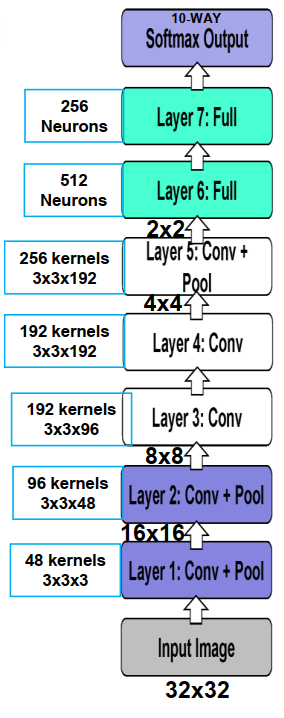
\includegraphics[scale=0.5]{image_0}
\end{center}
\end{flushleft}
\end{par}

\begin{matlabcode}
image_dim = [32 32 3];
kernel_dim = [3 3];
maxpool_dim = [2 2];
stride_conv_dim = [1 1];
stride_maxpool_dim = [2 2];

layers_1 = [
    imageInputLayer(image_dim, 'Name', 'data')
    
    convolution2dLayer(kernel_dim, 48, 'Name', 'conv1', 'BiasLearnRateFactor', 2, 'Stride', stride_conv_dim, 'Padding', 'same')
    reluLayer('Name','relu1')
    maxPooling2dLayer(maxpool_dim, 'Name', 'pool1', 'Stride', stride_maxpool_dim)
    
    convolution2dLayer(kernel_dim, 96, 'Name', 'conv2', 'BiasLearnRateFactor', 2, 'Stride', stride_conv_dim, 'Padding', 'same')
    reluLayer('Name','relu2')
    maxPooling2dLayer(maxpool_dim, 'Name', 'pool2', 'Stride', stride_maxpool_dim)
    
    convolution2dLayer(kernel_dim, 192, 'Name', 'conv3', 'BiasLearnRateFactor', 2, 'Stride', stride_conv_dim, 'Padding', 'same')
    reluLayer('Name','relu3')
    
    convolution2dLayer(kernel_dim, 192, 'Name', 'conv4', 'BiasLearnRateFactor', 2, 'Stride', stride_conv_dim, 'Padding', 'same')
    reluLayer('Name','relu4')
    maxPooling2dLayer(maxpool_dim, 'Name', 'pool4', 'Stride', stride_maxpool_dim)
    
    convolution2dLayer(kernel_dim, 256, 'Name', 'conv5', 'BiasLearnRateFactor', 2, 'Stride', stride_conv_dim, 'Padding', 'same')
    reluLayer('Name','relu5')
    maxPooling2dLayer(maxpool_dim, 'Name', 'pool5', 'Stride', stride_maxpool_dim)
    
    fullyConnectedLayer(512, 'Name', 'fc6', 'BiasLearnRateFactor', 2)
    reluLayer('Name', 'relu6')
    dropoutLayer(0.5,'Name','drop6')

    fullyConnectedLayer(256, 'Name', 'fc7', 'BiasLearnRateFactor', 2)
    reluLayer('Name','relu7')
    dropoutLayer(0.5,'Name','drop7')
    
    fullyConnectedLayer(10, 'Name', 'softmax', 'BiasLearnRateFactor', 2)
    softmaxLayer('Name','prob')
    
    classificationLayer('Name','output')
    ];

clear image_dim kernel_dim maxpool_dim stride_conv_dim stride_maxpool_dim

disp(layers_1);
\end{matlabcode}

\begin{matlaboutput}
  24x1 Layer array with layers:

     1   'data'      Image Input             32x32x3 images with 'zerocenter' normalization
     2   'conv1'     Convolution             48 3x3 convolutions with stride [1  1] and padding 'same'
     3   'relu1'     ReLU                    ReLU
     4   'pool1'     Max Pooling             2x2 max pooling with stride [2  2] and padding [0  0  0  0]
     5   'conv2'     Convolution             96 3x3 convolutions with stride [1  1] and padding 'same'
     6   'relu2'     ReLU                    ReLU
     7   'pool2'     Max Pooling             2x2 max pooling with stride [2  2] and padding [0  0  0  0]
     8   'conv3'     Convolution             192 3x3 convolutions with stride [1  1] and padding 'same'
     9   'relu3'     ReLU                    ReLU
    10   'conv4'     Convolution             192 3x3 convolutions with stride [1  1] and padding 'same'
    11   'relu4'     ReLU                    ReLU
    12   'pool4'     Max Pooling             2x2 max pooling with stride [2  2] and padding [0  0  0  0]
    13   'conv5'     Convolution             256 3x3 convolutions with stride [1  1] and padding 'same'
    14   'relu5'     ReLU                    ReLU
    15   'pool5'     Max Pooling             2x2 max pooling with stride [2  2] and padding [0  0  0  0]
    16   'fc6'       Fully Connected         512 fully connected layer
    17   'relu6'     ReLU                    ReLU
    18   'drop6'     Dropout                 50% dropout
    19   'fc7'       Fully Connected         256 fully connected layer
    20   'relu7'     ReLU                    ReLU
    21   'drop7'     Dropout                 50% dropout
    22   'softmax'   Fully Connected         10 fully connected layer
    23   'prob'      Softmax                 softmax
    24   'output'    Classification Output   crossentropyex
\end{matlaboutput}



\begin{par}
\begin{flushleft}
In the figure below, we can see the whole network at a glance:
\end{flushleft}
\end{par}

\begin{matlabcode}
%analyzeNetwork(layers_1);
plot(layerGraph(layers_1));
\end{matlabcode}
\begin{center}
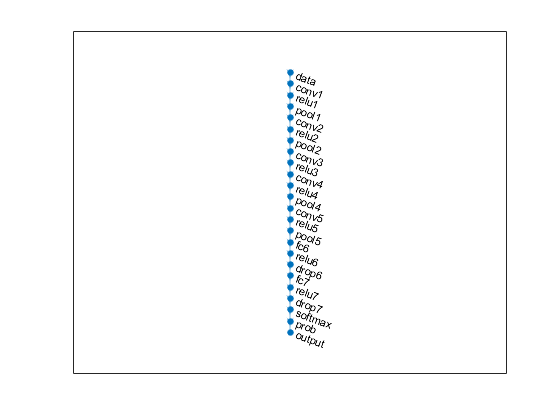
\includegraphics[scale=0.5]{figure_1.png}
\end{center}


\label{H_3C769346}
\matlabheading{1.3 Training the Network}

\label{H_422ACAD3}
\matlabheadingtwo{1.3.1 Split Training Data into \textit{train} and \textit{validation }Subsets}

\begin{par}
\begin{flushleft}
15 percent of the 50,000 training images are assigned to the validation set and the rest are kept for the neural network training.
\end{flushleft}
\end{par}

\begin{matlabcode}
[imdsTrain, imdsValidation] = splitEachLabel(imds,0.85,'randomized');
disp(countEachLabel(imdsTrain));
\end{matlabcode}
\begin{matlaboutput}
      Label       Count
    __________    _____

    airplane      4250 
    automobile    4250 
    bird          4250 
    cat           4250 
    deer          4250 
    dog           4250 
    frog          4250 
    horse         4250 
    ship          4250 
    truck         4250 
\end{matlaboutput}
\begin{matlabcode}
disp(countEachLabel(imdsValidation));
\end{matlabcode}
\begin{matlaboutput}
      Label       Count
    __________    _____

    airplane       750 
    automobile     750 
    bird           750 
    cat            750 
    deer           750 
    dog            750 
    frog           750 
    horse          750 
    ship           750 
    truck          750 
\end{matlaboutput}


\label{H_BD4FDDF6}
\matlabheadingtwo{1.3.2 Preprocessing the Training Data}

\begin{par}
\begin{flushleft}
To strengthen the training process and make the network invariant to distortions in images, we did some prerpocessnig on the training subset of the images, as listed below:
\end{flushleft}
\end{par}

\begin{itemize}
\setlength{\itemsep}{-1ex}
   \item{\begin{flushleft} Random reflection of images in the left-right direction with probability of 0.5 \end{flushleft}}
   \item{\begin{flushleft} Random horizontal translation picked from a continuous distribution of range [-3 3] \end{flushleft}}
   \item{\begin{flushleft} Random vertical translation picked from a continuous distribution of range [-3 3] \end{flushleft}}
\end{itemize}

\begin{matlabcode}
pixelRange = [-3 3];
imageAugmenter = imageDataAugmenter( ...
                    'RandXReflection',true, ...
                    'RandXTranslation',pixelRange, ...
                    'RandYTranslation',pixelRange);
augimdsTrain = augmentedImageDatastore([32 32], imdsTrain, ...
    'DataAugmentation',imageAugmenter);

\end{matlabcode}

\clearpage
\begin{par}
\begin{flushleft}
The first nine images before preprocessing:
\end{flushleft}
\end{par}

\begin{matlabcode}
montage(subset(imdsTrain, 1:9));
\end{matlabcode}
\begin{center}
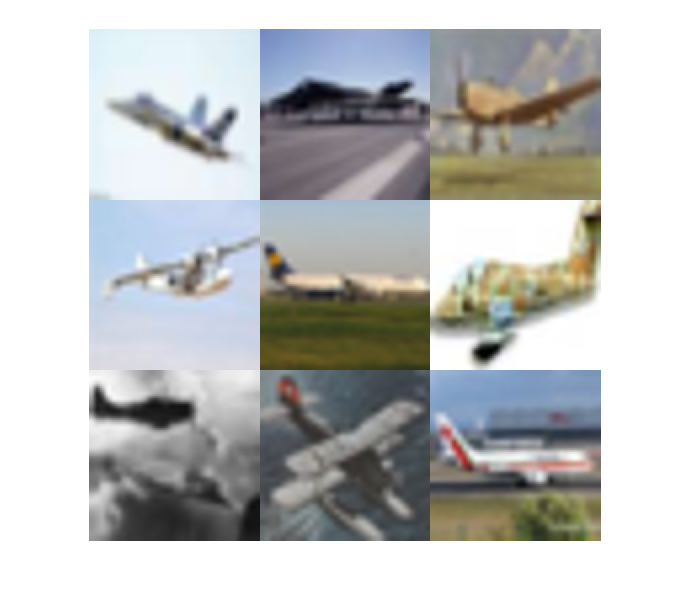
\includegraphics[scale=0.4]{figure_2.png}
\end{center}

\begin{par}
\begin{flushleft}
The first nine images after preprocessing:
\end{flushleft}
\end{par}

\begin{matlabcode}
montage(readByIndex(augimdsTrain, 1:9).input);
\end{matlabcode}
\begin{center}
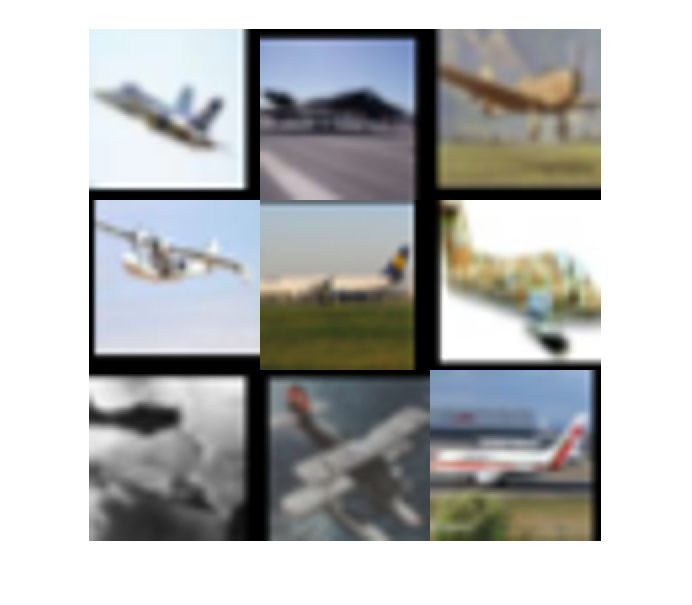
\includegraphics[scale=0.4]{figure_3.png}
\end{center}


\label{H_7638DD90}
\matlabheadingtwo{1.3.3 Defining Options for Training}

\begin{par}
\begin{flushleft}
We have used 40 epoches with mini-batch size of 512 and used the \textit{Adam} Optimizer.
\end{flushleft}
\end{par}

\begin{matlabcode}
opts = trainingOptions('adam', ...
    'ExecutionEnvironment','auto', ...
    'MaxEpochs', 40, ...
    'MiniBatchSize', 512, ...
    'Shuffle', 'every-epoch', ...
    'Plots', 'training-progress', ...
    'Verbose', true, ...
    'ValidationData', imdsValidation);
\end{matlabcode}


\label{H_26B8AACD}
\matlabheadingtwo{1.3.4 Learning Curves and Training Process}

\begin{par}
\begin{flushleft}
We trained the network on single GPU system nad print the results in a table every 50 iterations. Besides, the learning curves are plotted after the table. Finally the network reached 84.38\% on training and 81.37\% on validation subset. The training process took about 90 minutes long.
\end{flushleft}
\end{par}

\begin{matlabcode}
trained_net_1 = trainNetwork(augimdsTrain, layers_1, opts);
\end{matlabcode}

\begin{matlaboutput}
Warning: Support for GPU devices with Compute Capability 3.0 will be removed in a future MATLAB release. For more information on GPU support, see GPU Support by Release.
Training on single GPU.
Initializing input data normalization.
|===============================================================================================================|
|  Epoch  |  Iteration  |  Time Elapsed  |  Mini-batch  |  Validation  |  Mini-batch  |  Validation  |  Base Learning  |
|         |             |   (hh:mm:ss)   |   Accuracy   |   Accuracy   |     Loss     |     Loss     |      Rate       |
|===============================================================================================================|
|       1 |           1 |       00:02:46 |       10.55% |       10.00% |      11.1746 |       6.8502 |          0.0010 |
|       1 |          50 |       00:04:05 |       23.05% |       29.56% |       2.0305 |       1.9423 |          0.0010 |
|       2 |         100 |       00:05:24 |       31.84% |       38.39% |       1.8032 |       1.6916 |          0.0010 |
|       2 |         150 |       00:06:45 |       39.84% |       46.04% |       1.6340 |       1.4730 |          0.0010 |
|       3 |         200 |       00:08:05 |       48.44% |       48.04% |       1.4497 |       1.4095 |          0.0010 |
|       4 |         250 |       00:09:25 |       47.46% |       52.71% |       1.4264 |       1.3147 |          0.0010 |
|       4 |         300 |       00:10:45 |       51.95% |       56.84% |       1.3355 |       1.1858 |          0.0010 |
|       5 |         350 |       00:12:05 |       56.64% |       58.21% |       1.1940 |       1.1769 |          0.0010 |
|       5 |         400 |       00:13:26 |       56.05% |       60.15% |       1.2226 |       1.1227 |          0.0010 |
|       6 |         450 |       00:14:45 |       57.81% |       60.47% |       1.2050 |       1.1112 |          0.0010 |
|       7 |         500 |       00:16:06 |       64.84% |       64.23% |       1.0189 |       1.0050 |          0.0010 |
|       7 |         550 |       00:17:28 |       62.89% |       64.88% |       1.0022 |       0.9921 |          0.0010 |
|       8 |         600 |       00:18:49 |       65.43% |       67.41% |       1.0184 |       0.9291 |          0.0010 |
|       8 |         650 |       00:20:10 |       68.16% |       70.23% |       0.9114 |       0.8688 |          0.0010 |
|       9 |         700 |       00:21:31 |       71.48% |       68.93% |       0.8441 |       0.9062 |          0.0010 |
|      10 |         750 |       00:22:52 |       68.36% |       71.39% |       0.9565 |       0.8422 |          0.0010 |
|      10 |         800 |       00:24:13 |       67.19% |       70.61% |       0.9368 |       0.8515 |          0.0010 |
|      11 |         850 |       00:25:35 |       67.19% |       69.53% |       0.9207 |       0.8781 |          0.0010 |
|      11 |         900 |       00:26:55 |       71.48% |       70.40% |       0.8185 |       0.8636 |          0.0010 |
|      12 |         950 |       00:28:16 |       71.48% |       72.16% |       0.8344 |       0.8269 |          0.0010 |
|      13 |        1000 |       00:29:37 |       74.41% |       73.60% |       0.7181 |       0.7854 |          0.0010 |
|      13 |        1050 |       00:30:57 |       73.05% |       73.35% |       0.8046 |       0.7736 |          0.0010 |
|      14 |        1100 |       00:32:17 |       72.85% |       75.48% |       0.8163 |       0.7243 |          0.0010 |
|      14 |        1150 |       00:33:36 |       75.78% |       74.41% |       0.7186 |       0.7637 |          0.0010 |
|      15 |        1200 |       00:34:56 |       78.91% |       74.48% |       0.6884 |       0.7551 |          0.0010 |
|      16 |        1250 |       00:36:16 |       76.17% |       74.37% |       0.7158 |       0.7408 |          0.0010 |
|      16 |        1300 |       00:37:36 |       73.83% |       76.40% |       0.7440 |       0.7034 |          0.0010 |
|      17 |        1350 |       00:38:56 |       75.59% |       72.89% |       0.6730 |       0.7962 |          0.0010 |
|      17 |        1400 |       00:40:15 |       77.34% |       75.68% |       0.6674 |       0.7034 |          0.0010 |
|      18 |        1450 |       00:41:37 |       79.69% |       75.72% |       0.6195 |       0.7294 |          0.0010 |
|      19 |        1500 |       00:42:57 |       78.13% |       76.39% |       0.6104 |       0.6912 |          0.0010 |
|      19 |        1550 |       00:44:17 |       77.34% |       74.83% |       0.7288 |       0.7506 |          0.0010 |
|      20 |        1600 |       00:45:37 |       77.15% |       78.03% |       0.6956 |       0.6359 |          0.0010 |
|      20 |        1650 |       00:46:56 |       79.49% |       77.44% |       0.6096 |       0.6763 |          0.0010 |
|      21 |        1700 |       00:48:17 |       78.91% |       76.44% |       0.6358 |       0.6896 |          0.0010 |
|      22 |        1750 |       00:49:37 |       83.59% |       76.37% |       0.4726 |       0.7047 |          0.0010 |
|      22 |        1800 |       00:50:58 |       79.49% |       78.59% |       0.6246 |       0.6303 |          0.0010 |
|      23 |        1850 |       00:52:17 |       79.69% |       77.28% |       0.6480 |       0.6792 |          0.0010 |
|      23 |        1900 |       00:53:45 |       80.86% |       78.53% |       0.5494 |       0.6419 |          0.0010 |
|      24 |        1950 |       00:55:05 |       81.45% |       78.51% |       0.5932 |       0.6484 |          0.0010 |
|      25 |        2000 |       00:56:24 |       82.62% |       78.75% |       0.5143 |       0.6555 |          0.0010 |
|      25 |        2050 |       00:57:45 |       81.45% |       77.91% |       0.5461 |       0.6688 |          0.0010 |
|      26 |        2100 |       00:59:04 |       81.05% |       77.41% |       0.5522 |       0.6912 |          0.0010 |
|      26 |        2150 |       01:00:24 |       83.40% |       79.15% |       0.5004 |       0.6260 |          0.0010 |
|      27 |        2200 |       01:01:45 |       81.05% |       79.36% |       0.5271 |       0.6145 |          0.0010 |
|      28 |        2250 |       01:03:05 |       80.27% |       78.72% |       0.5737 |       0.6449 |          0.0010 |
|      28 |        2300 |       01:04:25 |       79.69% |       79.76% |       0.5618 |       0.6105 |          0.0010 |
|      29 |        2350 |       01:05:44 |       82.62% |       78.12% |       0.5440 |       0.6619 |          0.0010 |
|      29 |        2400 |       01:07:04 |       82.42% |       80.03% |       0.4902 |       0.6073 |          0.0010 |
|      30 |        2450 |       01:08:24 |       83.59% |       80.17% |       0.5028 |       0.5901 |          0.0010 |
|      31 |        2500 |       01:09:44 |       83.40% |       79.40% |       0.4549 |       0.6185 |          0.0010 |
|      31 |        2550 |       01:11:04 |       81.05% |       80.09% |       0.5590 |       0.6206 |          0.0010 |
|      32 |        2600 |       01:12:23 |       83.01% |       79.92% |       0.4975 |       0.6255 |          0.0010 |
|      32 |        2650 |       01:13:43 |       79.10% |       80.68% |       0.6294 |       0.5893 |          0.0010 |
|      33 |        2700 |       01:15:03 |       81.84% |       79.11% |       0.5202 |       0.6425 |          0.0010 |
|      34 |        2750 |       01:16:23 |       86.33% |       80.97% |       0.4711 |       0.5894 |          0.0010 |
|      34 |        2800 |       01:17:42 |       84.57% |       80.29% |       0.4627 |       0.6106 |          0.0010 |
|      35 |        2850 |       01:19:02 |       86.52% |       79.55% |       0.3983 |       0.6292 |          0.0010 |
|      35 |        2900 |       01:20:21 |       84.18% |       78.05% |       0.4886 |       0.6640 |          0.0010 |
|      36 |        2950 |       01:21:40 |       85.55% |       80.63% |       0.4258 |       0.6036 |          0.0010 |
|      37 |        3000 |       01:23:00 |       86.52% |       80.41% |       0.3825 |       0.6077 |          0.0010 |
|      37 |        3050 |       01:24:21 |       84.18% |       80.53% |       0.4640 |       0.6091 |          0.0010 |
|      38 |        3100 |       01:25:40 |       87.11% |       79.97% |       0.4125 |       0.6326 |          0.0010 |
|      38 |        3150 |       01:26:59 |       83.20% |       80.95% |       0.5435 |       0.5906 |          0.0010 |
|      39 |        3200 |       01:28:18 |       87.11% |       80.52% |       0.4022 |       0.6182 |          0.0010 |
|      40 |        3250 |       01:29:38 |       84.18% |       81.56% |       0.4500 |       0.5816 |          0.0010 |
|      40 |        3300 |       01:30:57 |       84.77% |       80.25% |       0.4485 |       0.6182 |          0.0010 |
|      40 |        3320 |       01:31:32 |       84.38% |       81.37% |       0.4713 |       0.5919 |          0.0010 |
|===============================================================================================================|
\end{matlaboutput}

\begin{center}
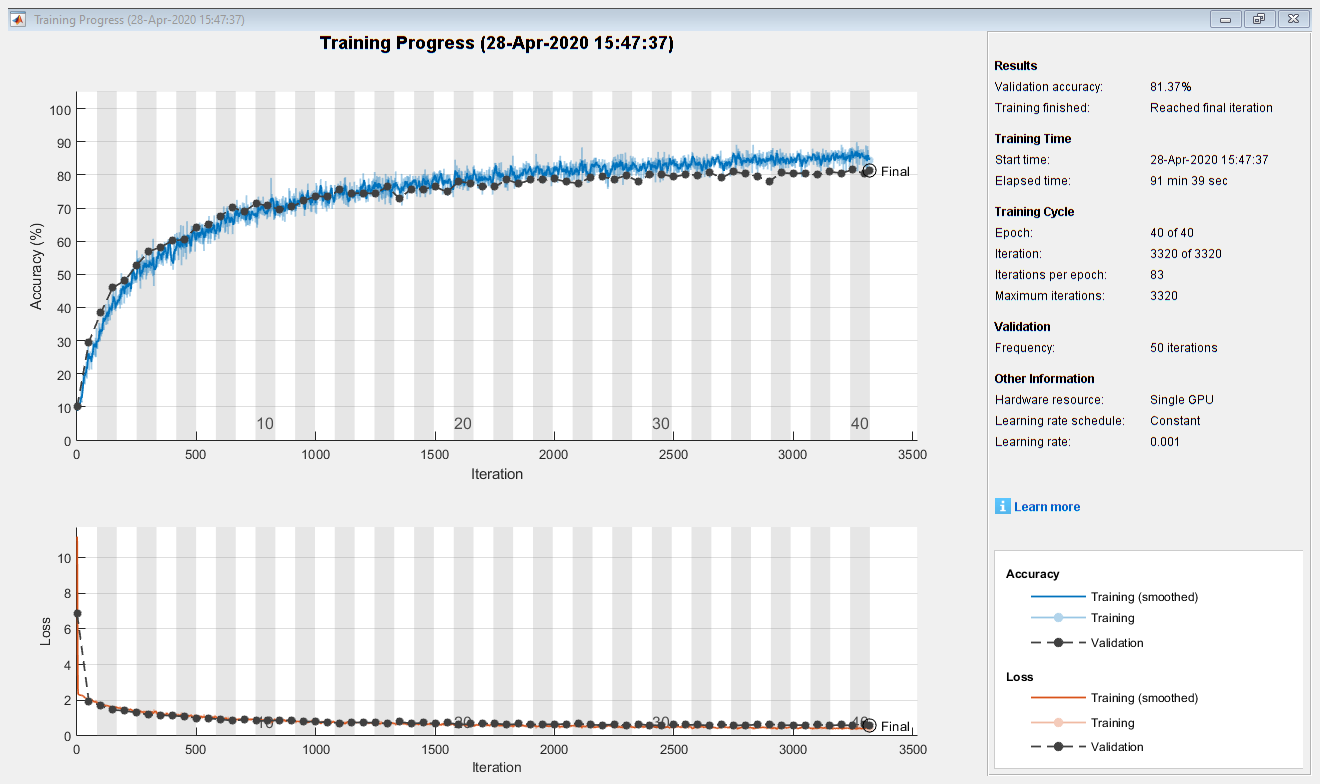
\includegraphics[width=\maxwidth{80.28098344204717em}]{figure_4.png}
\end{center}


\label{H_E1CF52CE}
\matlabheading{1.4 Evaluating the Network}

\begin{par}
\begin{flushleft}
Here we use the test partition of the dataset to evaluate the trained network.
\end{flushleft}
\end{par}

\label{H_6B1EDF81}
\matlabheadingtwo{1.4.1 Loading the Test Set of CIFAR-10}

\begin{matlabcode}
rootFolder = 'cifar10Test';
imds_test = imageDatastore(fullfile(rootFolder, categories), ...
    'LabelSource', 'foldernames');
clear rootFolder

disp(countEachLabel(imds_test));
\end{matlabcode}
\begin{matlaboutput}
      Label       Count
    __________    _____

    airplane      1000 
    automobile    1000 
    bird          1000 
    cat           1000 
    deer          1000 
    dog           1000 
    frog          1000 
    horse         1000 
    ship          1000 
    truck         1000 
\end{matlaboutput}


\label{H_0932904F}
\matlabheadingtwo{1.4.2 Classifying the Test Dataset}

\begin{par}
\begin{flushleft}
The line below will classify all images in the test dataset.
\end{flushleft}
\end{par}

\begin{matlabcode}
predicted_labels_1 = classify(trained_net_1, imds_test);
\end{matlabcode}


\label{H_C5596DFA}
\matlabheadingtwo{1.4.3 Plot Some Samples of the Test Dataset with the Predicted Label}

\begin{par}
\begin{flushleft}
Here we plot one sample of every class of the test dataset and display its predicted label on top of it. If it was predicted correctly the title will be in green color otherwise in red.
\end{flushleft}
\end{par}

\begin{matlabcode}
rand_nums = randi(size(imds_test.Files, 1)/10) + [0:1000:9000];

figure('Position', [100, 100, 1000, 1000]);
for i = 1:10
    if predicted_labels_1(rand_nums(i)) == imds_test.Labels(rand_nums(i))
        colorText = 'g'; 
    else
        colorText = 'r';
    end
    subplottight(3,4,i);
    imshow(imread(imds_test.Files{rand_nums(i)}));
    title(char(predicted_labels_1(rand_nums(i))), 'Color', colorText);
    hold on;
end
hold off
\end{matlabcode}
\begin{center}
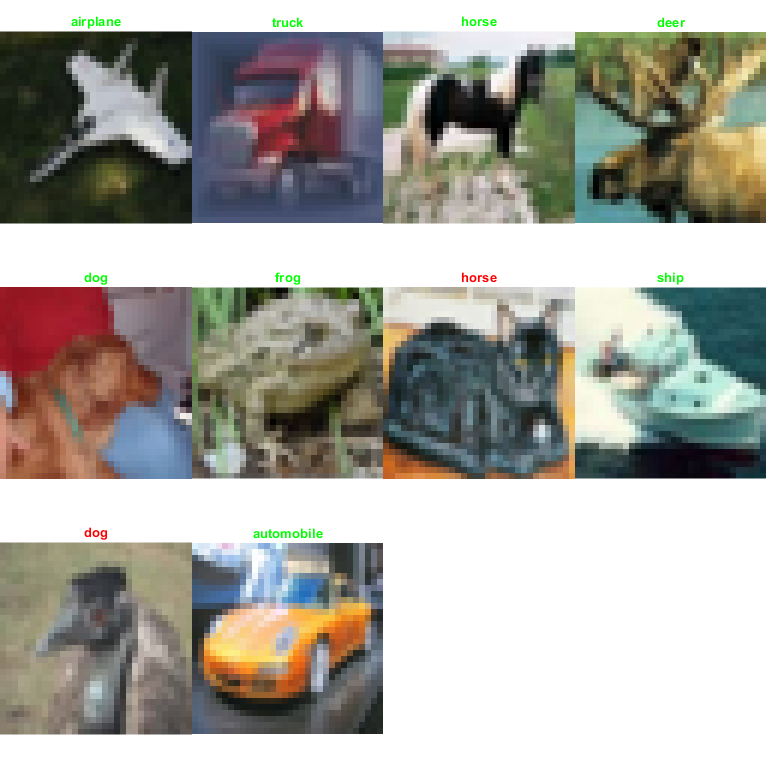
\includegraphics[scale=0.5]{figure_5.png}
\end{center}


\label{H_CB021FFA}
\matlabheadingtwo{1.4.4 Classification Performance}

\begin{par}
\begin{flushleft}
As the final step of this section, we plot the confusion matrix. Final performance of the network is 81.0\% over the whole test dataset.
\end{flushleft}
\end{par}

\begin{matlabcode}
plotconfusion(imds_test.Labels, predicted_labels_1);
\end{matlabcode}
\begin{center}
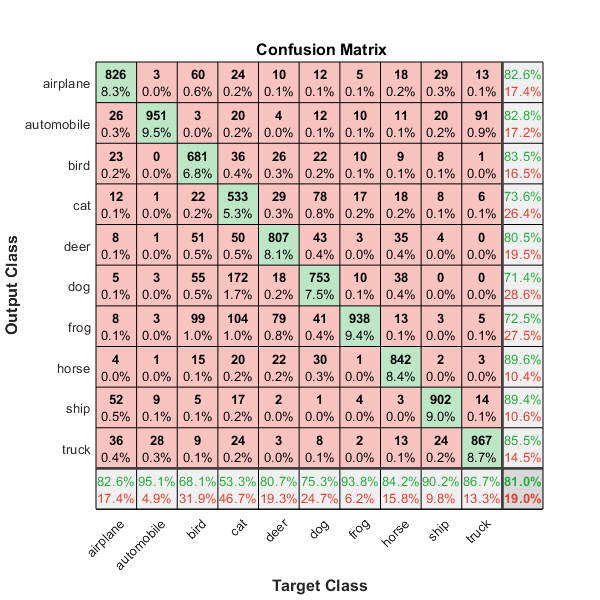
\includegraphics[scale=0.6]{figure_6.png}
\end{center}

\clearpage
\label{T_56C47E07}
\matlabtitle{2. Deleting Convolutional Layer 5 with Its Max-Pooling}

\label{H_CB48FECC}
\matlabheading{2.1 Defining Network Architecture }

\begin{par}
\begin{flushleft}
We define the layers of the network again as below. Convolutional layer 5 is deleted in comparison with question 1.
\end{flushleft}
\end{par}

\begin{matlabcode}
image_dim = [32 32 3];
kernel_dim = [3 3];
maxpool_dim = [2 2];
stride_conv_dim = [1 1];
stride_maxpool_dim = [2 2];

layers_2 = [
    imageInputLayer(image_dim, 'Name', 'data')
    
    convolution2dLayer(kernel_dim, 48, 'Name', 'conv1', 'BiasLearnRateFactor', 2, 'Stride', stride_conv_dim, 'Padding', 'same')
    reluLayer('Name','relu1')
    maxPooling2dLayer(maxpool_dim, 'Name', 'pool1', 'Stride', stride_maxpool_dim)
    
    convolution2dLayer(kernel_dim, 96, 'Name', 'conv2', 'BiasLearnRateFactor', 2, 'Stride', stride_conv_dim, 'Padding', 'same')
    reluLayer('Name','relu2')
    maxPooling2dLayer(maxpool_dim, 'Name', 'pool2', 'Stride', stride_maxpool_dim)
    
    convolution2dLayer(kernel_dim, 192, 'Name', 'conv3', 'BiasLearnRateFactor', 2, 'Stride', stride_conv_dim, 'Padding', 'same')
    reluLayer('Name','relu3')
    
    convolution2dLayer(kernel_dim, 192, 'Name', 'conv4', 'BiasLearnRateFactor', 2, 'Stride', stride_conv_dim, 'Padding', 'same')
    reluLayer('Name','relu4')
    maxPooling2dLayer(maxpool_dim, 'Name', 'pool4', 'Stride', stride_maxpool_dim)
    
    fullyConnectedLayer(512, 'Name', 'fc6', 'BiasLearnRateFactor', 2)
    reluLayer('Name', 'relu6')
    dropoutLayer(0.5,'Name','drop6')

    fullyConnectedLayer(256, 'Name', 'fc7', 'BiasLearnRateFactor', 2)
    reluLayer('Name','relu7')
    dropoutLayer(0.5,'Name','drop7')
    
    fullyConnectedLayer(10, 'Name', 'softmax', 'BiasLearnRateFactor', 2)
    softmaxLayer('Name','prob')
    
    classificationLayer('Name','output')
    ];

clear image_dim kernel_dim maxpool_dim stride_conv_dim stride_maxpool_dim

disp(layers_2);
\end{matlabcode}
\begin{matlaboutput}
  21x1 Layer array with layers:

     1   'data'      Image Input             32x32x3 images with 'zerocenter' normalization
     2   'conv1'     Convolution             48 3x3 convolutions with stride [1  1] and padding 'same'
     3   'relu1'     ReLU                    ReLU
     4   'pool1'     Max Pooling             2x2 max pooling with stride [2  2] and padding [0  0  0  0]
     5   'conv2'     Convolution             96 3x3 convolutions with stride [1  1] and padding 'same'
     6   'relu2'     ReLU                    ReLU
     7   'pool2'     Max Pooling             2x2 max pooling with stride [2  2] and padding [0  0  0  0]
     8   'conv3'     Convolution             192 3x3 convolutions with stride [1  1] and padding 'same'
     9   'relu3'     ReLU                    ReLU
    10   'conv4'     Convolution             192 3x3 convolutions with stride [1  1] and padding 'same'
    11   'relu4'     ReLU                    ReLU
    12   'pool4'     Max Pooling             2x2 max pooling with stride [2  2] and padding [0  0  0  0]
    13   'fc6'       Fully Connected         512 fully connected layer
    14   'relu6'     ReLU                    ReLU
    15   'drop6'     Dropout                 50% dropout
    16   'fc7'       Fully Connected         256 fully connected layer
    17   'relu7'     ReLU                    ReLU
    18   'drop7'     Dropout                 50% dropout
    19   'softmax'   Fully Connected         10 fully connected layer
    20   'prob'      Softmax                 softmax
    21   'output'    Classification Output   crossentropyex
\end{matlaboutput}


\begin{matlabcode}
%analyzeNetwork(layers_2);
plot(layerGraph(layers_2));
\end{matlabcode}
\begin{center}
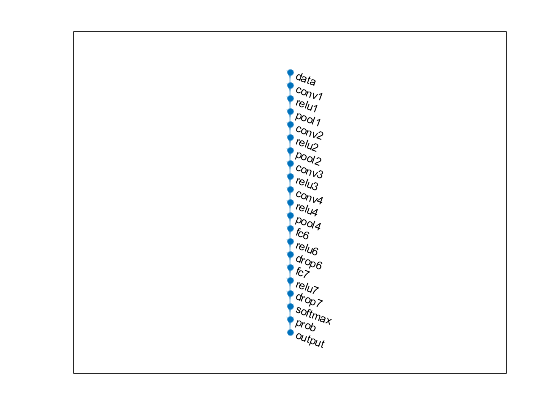
\includegraphics[scale=0.5]{figure_7.png}
\end{center}


\label{H_A8ABC5D4}
\matlabheading{2.2 Learning Curves and Training Process}

\begin{par}
\begin{flushleft}
We trained the network on single GPU system nad print the results in a table every 50 iterations. Besides, the learning curves are plotted after the table. Finally the network reached 83.59\% on training and 81.84\% on validation subset. The training process took about 90 minutes long.
\end{flushleft}
\end{par}

\begin{matlabcode}
trained_net_2 = trainNetwork(augimdsTrain, layers_2, opts);
\end{matlabcode}
\begin{matlaboutput}
Training on single GPU.
Initializing input data normalization.
|===============================================================================================================|
|  Epoch  |  Iteration  |  Time Elapsed  |  Mini-batch  |  Validation  |  Mini-batch  |  Validation  |  Base Learning  |
|         |             |   (hh:mm:ss)   |   Accuracy   |   Accuracy   |     Loss     |     Loss     |      Rate       |
|===============================================================================================================|
|       1 |           1 |       00:00:09 |        9.38% |       11.89% |      12.0610 |       7.1610 |          0.0010 |
|       1 |          50 |       00:01:17 |       24.61% |       28.69% |       2.0013 |       1.9260 |          0.0010 |
|       2 |         100 |       00:02:27 |       35.74% |       41.84% |       1.7440 |       1.6063 |          0.0010 |
|       2 |         150 |       00:03:36 |       38.28% |       44.99% |       1.6553 |       1.5126 |          0.0010 |
|       3 |         200 |       00:04:46 |       42.77% |       51.33% |       1.5858 |       1.3373 |          0.0010 |
|       4 |         250 |       00:05:56 |       50.98% |       52.97% |       1.3348 |       1.3207 |          0.0010 |
|       4 |         300 |       00:07:05 |       48.63% |       56.79% |       1.3816 |       1.2178 |          0.0010 |
|       5 |         350 |       00:08:15 |       56.45% |       56.97% |       1.2503 |       1.2198 |          0.0010 |
|       5 |         400 |       00:09:25 |       57.03% |       60.29% |       1.1812 |       1.1059 |          0.0010 |
|       6 |         450 |       00:10:34 |       58.98% |       62.77% |       1.1712 |       1.0679 |          0.0010 |
|       7 |         500 |       00:11:44 |       59.96% |       62.55% |       1.1371 |       1.1027 |          0.0010 |
|       7 |         550 |       00:12:54 |       61.52% |       65.28% |       1.1597 |       1.0064 |          0.0010 |
|       8 |         600 |       00:14:04 |       61.91% |       65.73% |       1.0565 |       0.9785 |          0.0010 |
|       8 |         650 |       00:15:18 |       63.48% |       66.64% |       1.0920 |       0.9404 |          0.0010 |
|       9 |         700 |       00:16:28 |       69.92% |       66.04% |       0.9164 |       0.9692 |          0.0010 |
|      10 |         750 |       00:17:38 |       66.60% |       69.52% |       0.9411 |       0.8815 |          0.0010 |
|      10 |         800 |       00:18:48 |       71.48% |       69.76% |       0.7699 |       0.8761 |          0.0010 |
|      11 |         850 |       00:20:00 |       65.23% |       70.47% |       0.9358 |       0.8700 |          0.0010 |
|      11 |         900 |       00:21:10 |       70.70% |       72.47% |       0.9084 |       0.8083 |          0.0010 |
|      12 |         950 |       00:22:19 |       68.36% |       71.25% |       0.8975 |       0.8242 |          0.0010 |
|      13 |        1000 |       00:23:28 |       68.55% |       71.35% |       0.8692 |       0.8445 |          0.0010 |
|      13 |        1050 |       00:24:38 |       73.44% |       73.73% |       0.8148 |       0.7670 |          0.0010 |
|      14 |        1100 |       00:25:49 |       73.63% |       72.89% |       0.7771 |       0.7887 |          0.0010 |
|      14 |        1150 |       00:29:23 |       76.17% |       75.27% |       0.7079 |       0.7233 |          0.0010 |
|      15 |        1200 |       00:31:07 |       71.48% |       73.53% |       0.8016 |       0.7810 |          0.0010 |
|      16 |        1250 |       00:32:16 |       73.24% |       74.20% |       0.7701 |       0.7504 |          0.0010 |
|      16 |        1300 |       00:33:26 |       75.78% |       75.41% |       0.6784 |       0.7155 |          0.0010 |
|      17 |        1350 |       00:34:35 |       76.76% |       73.65% |       0.6671 |       0.7765 |          0.0010 |
|      17 |        1400 |       00:35:44 |       77.54% |       75.12% |       0.6493 |       0.7253 |          0.0010 |
|      18 |        1450 |       00:36:54 |       74.61% |       75.76% |       0.7402 |       0.7145 |          0.0010 |
|      19 |        1500 |       00:38:03 |       76.56% |       75.68% |       0.6916 |       0.7319 |          0.0010 |
|      19 |        1550 |       00:39:13 |       73.83% |       77.16% |       0.7549 |       0.6655 |          0.0010 |
|      20 |        1600 |       00:40:22 |       76.37% |       75.81% |       0.6699 |       0.6971 |          0.0010 |
|      20 |        1650 |       00:41:32 |       80.86% |       76.53% |       0.5834 |       0.7003 |          0.0010 |
|      21 |        1700 |       00:42:42 |       77.15% |       76.93% |       0.6758 |       0.6791 |          0.0010 |
|      22 |        1750 |       00:43:51 |       81.05% |       77.19% |       0.5636 |       0.6791 |          0.0010 |
|      22 |        1800 |       00:45:01 |       75.00% |       77.51% |       0.7534 |       0.6539 |          0.0010 |
|      23 |        1850 |       00:46:10 |       78.13% |       76.97% |       0.6281 |       0.6714 |          0.0010 |
|      23 |        1900 |       00:47:20 |       75.39% |       77.09% |       0.7354 |       0.6630 |          0.0010 |
|      24 |        1950 |       00:48:29 |       80.86% |       77.93% |       0.5824 |       0.6567 |          0.0010 |
|      25 |        2000 |       00:49:38 |       79.88% |       78.03% |       0.6081 |       0.6421 |          0.0010 |
|      25 |        2050 |       00:50:47 |       76.37% |       79.05% |       0.6632 |       0.6310 |          0.0010 |
|      26 |        2100 |       00:51:57 |       81.05% |       78.31% |       0.5620 |       0.6360 |          0.0010 |
|      26 |        2150 |       00:53:06 |       75.98% |       77.65% |       0.7153 |       0.6562 |          0.0010 |
|      27 |        2200 |       00:54:15 |       79.69% |       79.37% |       0.5905 |       0.6066 |          0.0010 |
|      28 |        2250 |       00:55:24 |       80.47% |       79.25% |       0.5553 |       0.6123 |          0.0010 |
|      28 |        2300 |       00:56:33 |       84.38% |       78.88% |       0.4753 |       0.6269 |          0.0010 |
|      29 |        2350 |       00:57:43 |       79.30% |       79.51% |       0.5687 |       0.6096 |          0.0010 |
|      29 |        2400 |       00:58:52 |       79.69% |       80.08% |       0.5822 |       0.5920 |          0.0010 |
|      30 |        2450 |       01:00:01 |       81.64% |       79.64% |       0.5390 |       0.6008 |          0.0010 |
|      31 |        2500 |       01:01:10 |       83.40% |       80.20% |       0.4910 |       0.5718 |          0.0010 |
|      31 |        2550 |       01:02:19 |       82.42% |       78.44% |       0.5220 |       0.6315 |          0.0010 |
|      32 |        2600 |       01:03:28 |       80.47% |       79.51% |       0.5769 |       0.6148 |          0.0010 |
|      32 |        2650 |       01:04:38 |       80.08% |       80.07% |       0.5332 |       0.5917 |          0.0010 |
|      33 |        2700 |       01:05:47 |       81.05% |       79.80% |       0.5771 |       0.6039 |          0.0010 |
|      34 |        2750 |       01:06:56 |       81.64% |       80.25% |       0.5067 |       0.5886 |          0.0010 |
|      34 |        2800 |       01:08:05 |       79.10% |       80.00% |       0.5623 |       0.5812 |          0.0010 |
|      35 |        2850 |       01:09:15 |       84.77% |       80.63% |       0.4710 |       0.5896 |          0.0010 |
|      35 |        2900 |       01:10:24 |       81.64% |       79.89% |       0.5543 |       0.5858 |          0.0010 |
|      36 |        2950 |       01:11:33 |       82.81% |       80.01% |       0.5047 |       0.6002 |          0.0010 |
|      37 |        3000 |       01:12:42 |       83.40% |       81.03% |       0.4941 |       0.5815 |          0.0010 |
|      37 |        3050 |       01:13:52 |       82.03% |       81.28% |       0.4730 |       0.5653 |          0.0010 |
|      38 |        3100 |       01:15:01 |       83.20% |       79.64% |       0.5356 |       0.6305 |          0.0010 |
|      38 |        3150 |       01:16:10 |       85.74% |       80.91% |       0.4294 |       0.5786 |          0.0010 |
|      39 |        3200 |       01:17:19 |       84.38% |       78.64% |       0.4582 |       0.6789 |          0.0010 |
|      40 |        3250 |       01:18:28 |       83.40% |       79.57% |       0.4886 |       0.6115 |          0.0010 |
|      40 |        3300 |       01:19:38 |       83.20% |       81.63% |       0.4353 |       0.5549 |          0.0010 |
|      40 |        3320 |       01:20:10 |       83.59% |       81.84% |       0.4765 |       0.5440 |          0.0010 |
|===============================================================================================================|
\end{matlaboutput}
\begin{center}
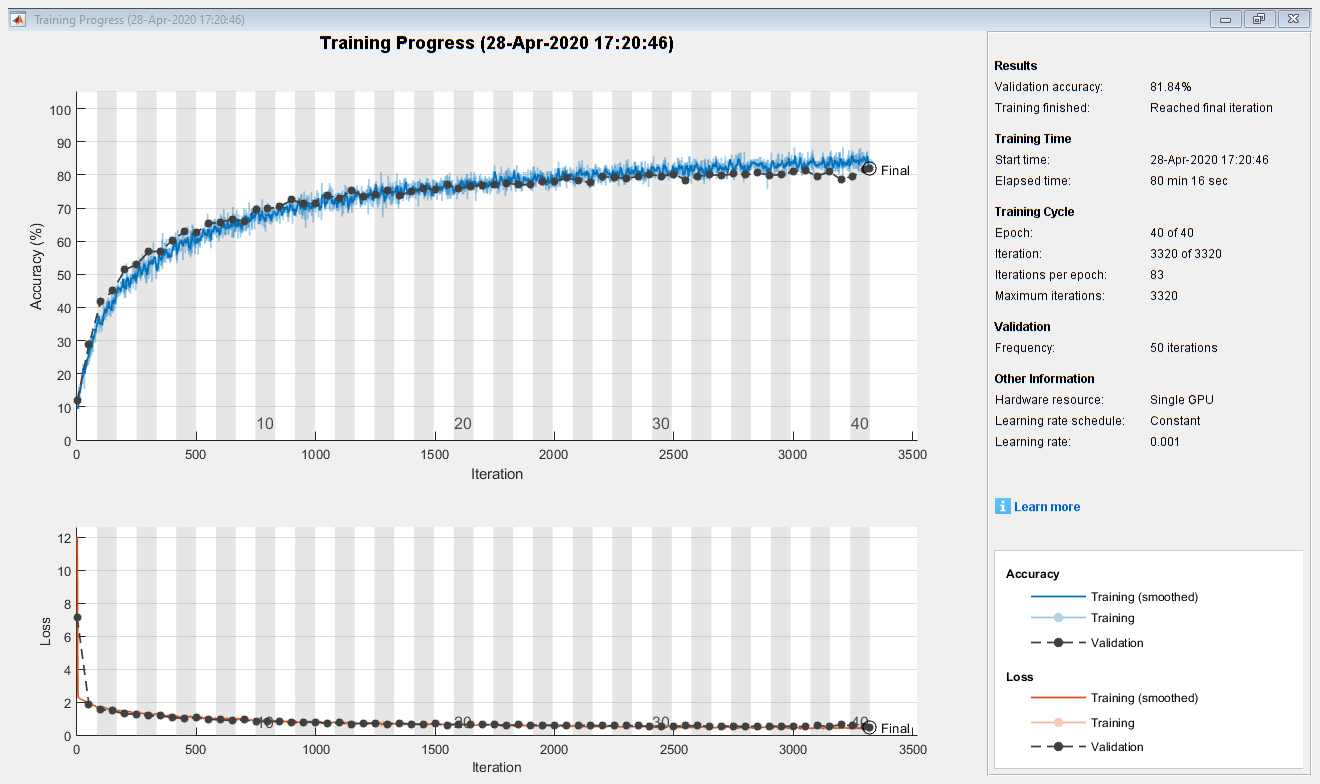
\includegraphics[width=\maxwidth{80.28098344204717em}]{figure_8.png}
\end{center}


\label{H_5F1379EF}
\matlabheading{2.3 Evaluating the Network}

\begin{par}
\begin{flushleft}
Here we use the test partition of the dataset to evaluate the trained network.
\end{flushleft}
\end{par}

\label{H_BB9EDA83}
\matlabheadingtwo{2.3.1 Classifying the Test Dataset}

\begin{par}
\begin{flushleft}
The line below will classify all images in the test dataset.
\end{flushleft}
\end{par}

\begin{matlabcode}
predicted_labels_2 = classify(trained_net_2, imds_test);
\end{matlabcode}


\label{H_B90267C9}
\matlabheadingtwo{2.3.2 Classification Performance}

\begin{par}
\begin{flushleft}
As the final step of this section, we plot the confusion matrix. The final performance of the network is 81.7\% over the whole test dataset.
\end{flushleft}
\end{par}

\begin{matlabcode}
plotconfusion(imds_test.Labels, predicted_labels_2);
\end{matlabcode}
\begin{center}
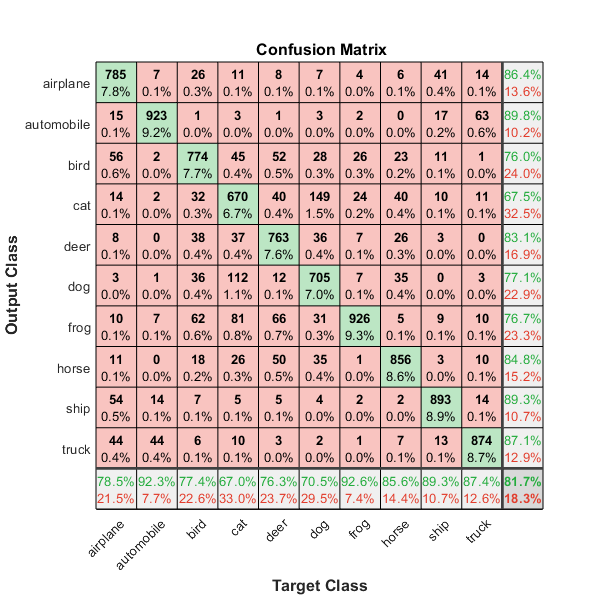
\includegraphics[scale=0.6]{figure_9.png}
\end{center}

\clearpage
\label{T_E008CB32}
\matlabtitle{3. Deleting Convolutional Layer 4 with Its Max-Pooling}

\label{H_857CBEBE}
\matlabheading{3.1 Defining Network Architecture }

\begin{par}
\begin{flushleft}
We define the layers of the network again as below. Convolutional layer 4 is deleted in comparison with question 1.
\end{flushleft}
\end{par}

\begin{matlabcode}
image_dim = [32 32 3];
kernel_dim = [3 3];
maxpool_dim = [2 2];
stride_conv_dim = [1 1];
stride_maxpool_dim = [2 2];

layers_3 = [
    imageInputLayer(image_dim, 'Name', 'data')
    
    convolution2dLayer(kernel_dim, 48, 'Name', 'conv1', 'BiasLearnRateFactor', 2, 'Stride', stride_conv_dim, 'Padding', 'same')
    reluLayer('Name','relu1')
    maxPooling2dLayer(maxpool_dim, 'Name', 'pool1', 'Stride', stride_maxpool_dim)
    
    convolution2dLayer(kernel_dim, 96, 'Name', 'conv2', 'BiasLearnRateFactor', 2, 'Stride', stride_conv_dim, 'Padding', 'same')
    reluLayer('Name','relu2')
    maxPooling2dLayer(maxpool_dim, 'Name', 'pool2', 'Stride', stride_maxpool_dim)
    
    convolution2dLayer(kernel_dim, 192, 'Name', 'conv3', 'BiasLearnRateFactor', 2, 'Stride', stride_conv_dim, 'Padding', 'same')
    reluLayer('Name','relu3')
    
    convolution2dLayer(kernel_dim, 256, 'Name', 'conv5', 'BiasLearnRateFactor', 2, 'Stride', stride_conv_dim, 'Padding', 'same')
    reluLayer('Name','relu5')
    maxPooling2dLayer(maxpool_dim, 'Name', 'pool5', 'Stride', stride_maxpool_dim)
    
    fullyConnectedLayer(512, 'Name', 'fc6', 'BiasLearnRateFactor', 2)
    reluLayer('Name', 'relu6')
    dropoutLayer(0.5,'Name','drop6')

    fullyConnectedLayer(256, 'Name', 'fc7', 'BiasLearnRateFactor', 2)
    reluLayer('Name','relu7')
    dropoutLayer(0.5,'Name','drop7')
    
    fullyConnectedLayer(10, 'Name', 'softmax', 'BiasLearnRateFactor', 2)
    softmaxLayer('Name','prob')
    
    classificationLayer('Name','output')
    ];

clear image_dim kernel_dim maxpool_dim stride_conv_dim stride_maxpool_dim

disp(layers_3);
\end{matlabcode}
\begin{matlaboutput}
  21x1 Layer array with layers:

     1   'data'      Image Input             32x32x3 images with 'zerocenter' normalization
     2   'conv1'     Convolution             48 3x3 convolutions with stride [1  1] and padding 'same'
     3   'relu1'     ReLU                    ReLU
     4   'pool1'     Max Pooling             2x2 max pooling with stride [2  2] and padding [0  0  0  0]
     5   'conv2'     Convolution             96 3x3 convolutions with stride [1  1] and padding 'same'
     6   'relu2'     ReLU                    ReLU
     7   'pool2'     Max Pooling             2x2 max pooling with stride [2  2] and padding [0  0  0  0]
     8   'conv3'     Convolution             192 3x3 convolutions with stride [1  1] and padding 'same'
     9   'relu3'     ReLU                    ReLU
    10   'conv5'     Convolution             256 3x3 convolutions with stride [1  1] and padding 'same'
    11   'relu5'     ReLU                    ReLU
    12   'pool5'     Max Pooling             2x2 max pooling with stride [2  2] and padding [0  0  0  0]
    13   'fc6'       Fully Connected         512 fully connected layer
    14   'relu6'     ReLU                    ReLU
    15   'drop6'     Dropout                 50% dropout
    16   'fc7'       Fully Connected         256 fully connected layer
    17   'relu7'     ReLU                    ReLU
    18   'drop7'     Dropout                 50% dropout
    19   'softmax'   Fully Connected         10 fully connected layer
    20   'prob'      Softmax                 softmax
    21   'output'    Classification Output   crossentropyex
\end{matlaboutput}


\begin{matlabcode}
%analyzeNetwork(layers_3);
plot(layerGraph(layers_3));
\end{matlabcode}
\begin{center}
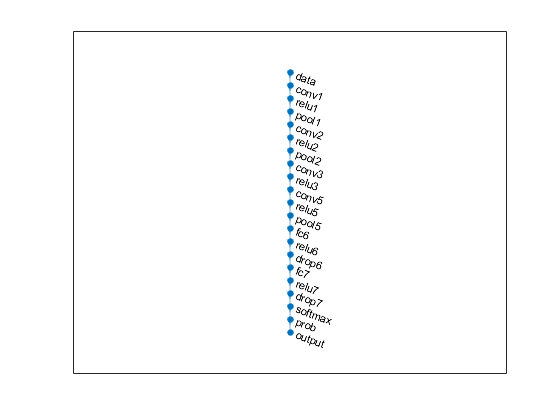
\includegraphics[scale=0.5]{figure_10.png}
\end{center}


\label{H_8767FA72}
\matlabheading{3.2 Learning Curves and Training Process}

\begin{par}
\begin{flushleft}
We trained the network on single GPU system nad print the results in a table every 50 iterations. Besides, the learning curves are plotted after the table. Finally the network reached 83.59\% on training and 81.17\% on validation subset. The training process took about 90 minutes long.
\end{flushleft}
\end{par}

\begin{matlabcode}
trained_net_3 = trainNetwork(augimdsTrain, layers_3, opts);
\end{matlabcode}
\begin{matlaboutput}
Training on single GPU.
Initializing input data normalization.
|===============================================================================================================|
|  Epoch  |  Iteration  |  Time Elapsed  |  Mini-batch  |  Validation  |  Mini-batch  |  Validation  |  Base Learning  |
|         |             |   (hh:mm:ss)   |   Accuracy   |   Accuracy   |     Loss     |     Loss     |      Rate       |
|===============================================================================================================|
|       1 |           1 |       00:00:09 |        8.40% |       10.51% |      12.4558 |       7.5910 |          0.0010 |
|       1 |          50 |       00:01:22 |       25.98% |       34.25% |       1.9766 |       1.8403 |          0.0010 |
|       2 |         100 |       00:02:36 |       33.20% |       41.79% |       1.7935 |       1.6030 |          0.0010 |
|       2 |         150 |       00:03:50 |       37.50% |       44.89% |       1.7270 |       1.5264 |          0.0010 |
|       3 |         200 |       00:05:04 |       44.34% |       50.48% |       1.5197 |       1.3583 |          0.0010 |
|       4 |         250 |       00:06:18 |       49.61% |       50.32% |       1.4239 |       1.3820 |          0.0010 |
|       4 |         300 |       00:07:32 |       50.00% |       57.88% |       1.3442 |       1.1852 |          0.0010 |
|       5 |         350 |       00:08:46 |       56.45% |       59.64% |       1.2219 |       1.1483 |          0.0010 |
|       5 |         400 |       00:10:02 |       57.03% |       59.75% |       1.2362 |       1.1274 |          0.0010 |
|       6 |         450 |       00:11:17 |       56.64% |       61.13% |       1.2024 |       1.1178 |          0.0010 |
|       7 |         500 |       00:12:31 |       61.91% |       61.68% |       1.1280 |       1.0773 |          0.0010 |
|       7 |         550 |       00:13:46 |       64.06% |       66.67% |       1.0673 |       0.9591 |          0.0010 |
|       8 |         600 |       00:15:00 |       65.04% |       66.17% |       1.0417 |       0.9873 |          0.0010 |
|       8 |         650 |       00:16:15 |       65.63% |       63.72% |       1.0807 |       1.0454 |          0.0010 |
|       9 |         700 |       00:17:30 |       67.19% |       68.00% |       0.9540 |       0.9266 |          0.0010 |
|      10 |         750 |       00:18:44 |       67.19% |       66.24% |       0.9907 |       0.9674 |          0.0010 |
|      10 |         800 |       00:19:59 |       67.19% |       69.32% |       0.9006 |       0.8895 |          0.0010 |
|      11 |         850 |       00:21:13 |       68.55% |       71.21% |       1.0141 |       0.8429 |          0.0010 |
|      11 |         900 |       00:22:28 |       67.19% |       72.00% |       0.9094 |       0.8113 |          0.0010 |
|      12 |         950 |       00:23:42 |       72.07% |       71.45% |       0.7779 |       0.8314 |          0.0010 |
|      13 |        1000 |       00:24:56 |       69.53% |       71.87% |       0.8481 |       0.8128 |          0.0010 |
|      13 |        1050 |       00:26:11 |       71.29% |       70.47% |       0.7981 |       0.8714 |          0.0010 |
|      14 |        1100 |       00:27:25 |       74.02% |       72.20% |       0.7570 |       0.8164 |          0.0010 |
|      14 |        1150 |       00:28:40 |       73.24% |       73.76% |       0.7977 |       0.7711 |          0.0010 |
|      15 |        1200 |       00:29:54 |       73.63% |       74.25% |       0.7361 |       0.7520 |          0.0010 |
|      16 |        1250 |       00:31:08 |       77.73% |       74.15% |       0.6777 |       0.7562 |          0.0010 |
|      16 |        1300 |       00:32:22 |       72.66% |       75.37% |       0.8078 |       0.7201 |          0.0010 |
|      17 |        1350 |       00:33:36 |       75.59% |       75.68% |       0.7724 |       0.7068 |          0.0010 |
|      17 |        1400 |       00:34:50 |       75.98% |       76.27% |       0.7133 |       0.7029 |          0.0010 |
|      18 |        1450 |       00:36:04 |       75.20% |       76.87% |       0.7074 |       0.6885 |          0.0010 |
|      19 |        1500 |       00:37:18 |       71.48% |       77.04% |       0.7779 |       0.6740 |          0.0010 |
|      19 |        1550 |       00:38:32 |       75.98% |       76.57% |       0.6821 |       0.6965 |          0.0010 |
|      20 |        1600 |       00:39:46 |       78.71% |       75.57% |       0.6723 |       0.7495 |          0.0010 |
|      20 |        1650 |       00:41:00 |       76.17% |       77.03% |       0.6501 |       0.6822 |          0.0010 |
|      21 |        1700 |       00:42:14 |       77.73% |       76.61% |       0.6755 |       0.6961 |          0.0010 |
|      22 |        1750 |       00:43:29 |       80.47% |       76.69% |       0.5903 |       0.6787 |          0.0010 |
|      22 |        1800 |       00:44:43 |       78.71% |       78.53% |       0.6083 |       0.6350 |          0.0010 |
|      23 |        1850 |       00:45:57 |       76.76% |       76.88% |       0.7153 |       0.6905 |          0.0010 |
|      23 |        1900 |       00:47:11 |       76.56% |       78.25% |       0.6748 |       0.6467 |          0.0010 |
|      24 |        1950 |       00:48:25 |       81.84% |       78.13% |       0.5674 |       0.6835 |          0.0010 |
|      25 |        2000 |       00:49:39 |       78.71% |       78.07% |       0.5549 |       0.6560 |          0.0010 |
|      25 |        2050 |       00:50:53 |       80.86% |       78.41% |       0.5516 |       0.6459 |          0.0010 |
|      26 |        2100 |       00:52:08 |       79.69% |       77.97% |       0.6324 |       0.6510 |          0.0010 |
|      26 |        2150 |       00:53:22 |       78.32% |       78.12% |       0.6190 |       0.6611 |          0.0010 |
|      27 |        2200 |       00:54:36 |       81.64% |       78.71% |       0.5365 |       0.6301 |          0.0010 |
|      28 |        2250 |       00:55:51 |       77.73% |       77.92% |       0.6132 |       0.6678 |          0.0010 |
|      28 |        2300 |       00:57:05 |       80.66% |       78.64% |       0.5374 |       0.6289 |          0.0010 |
|      29 |        2350 |       00:58:19 |       81.05% |       79.95% |       0.6034 |       0.6107 |          0.0010 |
|      29 |        2400 |       00:59:34 |       85.74% |       78.45% |       0.4658 |       0.6574 |          0.0010 |
|      30 |        2450 |       01:00:48 |       80.66% |       79.41% |       0.5758 |       0.6080 |          0.0010 |
|      31 |        2500 |       01:02:03 |       82.81% |       79.09% |       0.5239 |       0.6284 |          0.0010 |
|      31 |        2550 |       01:03:17 |       82.42% |       79.73% |       0.5658 |       0.6017 |          0.0010 |
|      32 |        2600 |       01:04:31 |       81.05% |       80.19% |       0.5426 |       0.6025 |          0.0010 |
|      32 |        2650 |       01:05:46 |       82.03% |       79.59% |       0.5275 |       0.6171 |          0.0010 |
|      33 |        2700 |       01:07:00 |       82.81% |       81.12% |       0.5312 |       0.5785 |          0.0010 |
|      34 |        2750 |       01:08:15 |       80.47% |       79.36% |       0.5784 |       0.6150 |          0.0010 |
|      34 |        2800 |       01:09:29 |       79.69% |       79.77% |       0.5607 |       0.6057 |          0.0010 |
|      35 |        2850 |       01:10:43 |       82.42% |       78.88% |       0.4991 |       0.6532 |          0.0010 |
|      35 |        2900 |       01:11:58 |       81.45% |       80.77% |       0.5652 |       0.5843 |          0.0010 |
|      36 |        2950 |       01:13:12 |       82.03% |       81.05% |       0.5043 |       0.5763 |          0.0010 |
|      37 |        3000 |       01:14:26 |       85.16% |       80.87% |       0.4620 |       0.5881 |          0.0010 |
|      37 |        3050 |       01:15:40 |       81.84% |       80.83% |       0.5218 |       0.5819 |          0.0010 |
|      38 |        3100 |       01:16:56 |       85.35% |       80.88% |       0.4086 |       0.5834 |          0.0010 |
|      38 |        3150 |       01:18:10 |       83.79% |       81.27% |       0.4887 |       0.5780 |          0.0010 |
|      39 |        3200 |       01:19:25 |       81.25% |       81.44% |       0.5146 |       0.6004 |          0.0010 |
|      40 |        3250 |       01:20:40 |       82.03% |       81.45% |       0.4769 |       0.5755 |          0.0010 |
|      40 |        3300 |       01:21:54 |       84.38% |       81.43% |       0.4589 |       0.5587 |          0.0010 |
|      40 |        3320 |       01:22:28 |       83.59% |       81.17% |       0.4991 |       0.5806 |          0.0010 |
|===============================================================================================================|
\end{matlaboutput}
\begin{center}
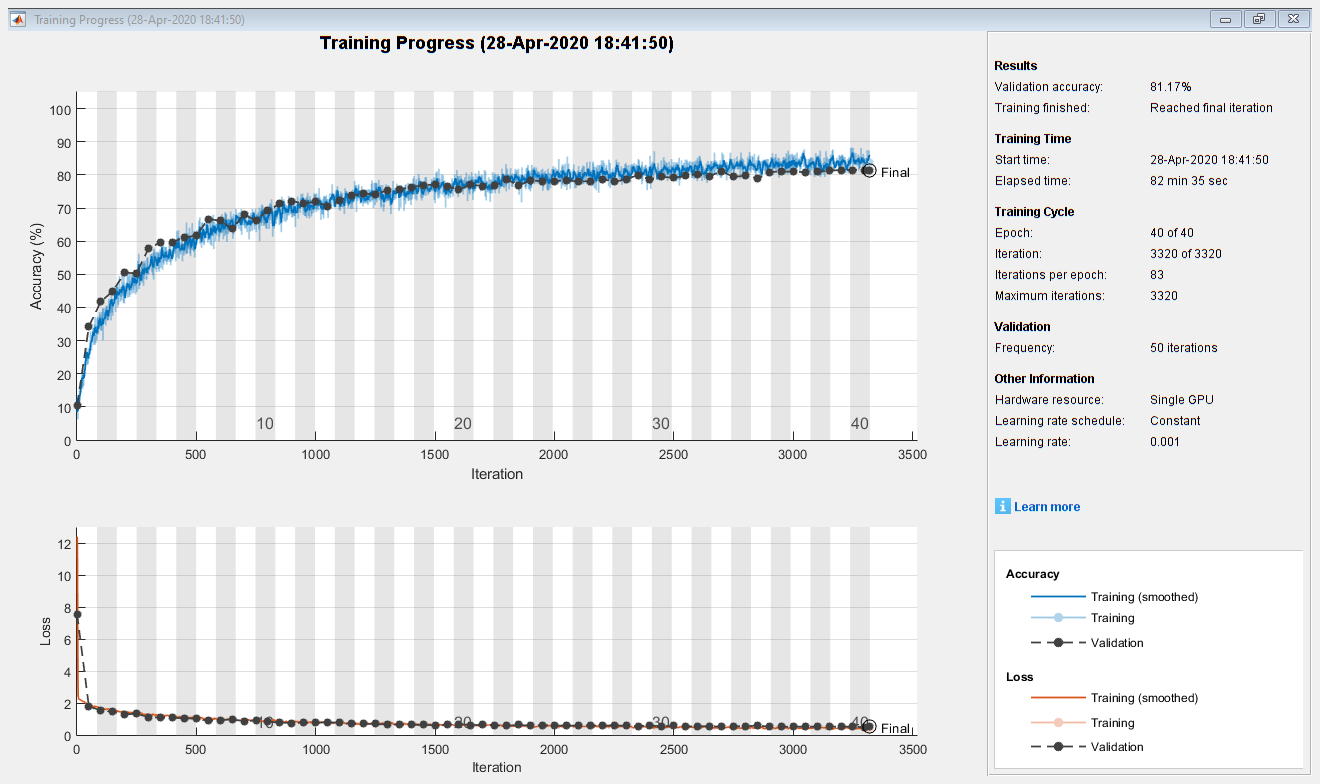
\includegraphics[width=\maxwidth{80.28098344204717em}]{figure_11.png}
\end{center}


\label{H_46DD8C17}
\matlabheading{3.3 Evaluating the Network}

\begin{par}
\begin{flushleft}
Here we use the test partition of the dataset to evaluate the trained network.
\end{flushleft}
\end{par}

\label{H_521F9240}
\matlabheadingtwo{3.3.1 Classifying the Test Dataset}

\begin{par}
\begin{flushleft}
The line below will classify all images in the test dataset.
\end{flushleft}
\end{par}

\begin{matlabcode}
predicted_labels_3 = classify(trained_net_3, imds_test);
\end{matlabcode}


\label{H_114CC648}
\matlabheadingtwo{3.3.2 Classification Performance}

\begin{par}
\begin{flushleft}
As the final step of this section, we plot the confusion matrix. The final performance of the network is 80.8\% over the whole test dataset.
\end{flushleft}
\end{par}

\begin{matlabcode}
plotconfusion(imds_test.Labels, predicted_labels_3);
\end{matlabcode}
\begin{center}
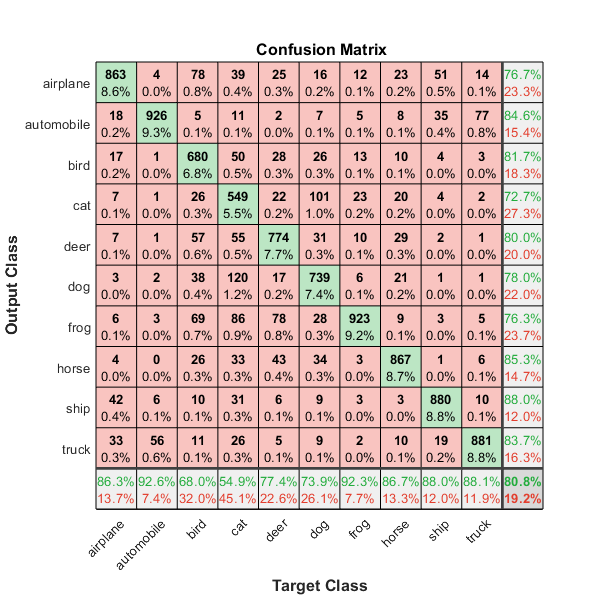
\includegraphics[scale=0.6]{figure_12.png}
\end{center}

\clearpage
\label{T_57C869E5}
\matlabtitle{4. Deleting Fully-Connected Layer 6}

\label{H_838E75A7}
\matlabheading{4.1 Defining Network Architecture }

\begin{par}
\begin{flushleft}
We define the layers of the network again as below. Fully-Connected layer 6 is deleted in comparison with question 1.
\end{flushleft}
\end{par}

\begin{matlabcode}
image_dim = [32 32 3];
kernel_dim = [3 3];
maxpool_dim = [2 2];
stride_conv_dim = [1 1];
stride_maxpool_dim = [2 2];

layers_4 = [
    imageInputLayer(image_dim, 'Name', 'data')
    
    convolution2dLayer(kernel_dim, 48, 'Name', 'conv1', 'BiasLearnRateFactor', 2, 'Stride', stride_conv_dim, 'Padding', 'same')
    reluLayer('Name','relu1')
    maxPooling2dLayer(maxpool_dim, 'Name', 'pool1', 'Stride', stride_maxpool_dim)
    
    convolution2dLayer(kernel_dim, 96, 'Name', 'conv2', 'BiasLearnRateFactor', 2, 'Stride', stride_conv_dim, 'Padding', 'same')
    reluLayer('Name','relu2')
    maxPooling2dLayer(maxpool_dim, 'Name', 'pool2', 'Stride', stride_maxpool_dim)
    
    convolution2dLayer(kernel_dim, 192, 'Name', 'conv3', 'BiasLearnRateFactor', 2, 'Stride', stride_conv_dim, 'Padding', 'same')
    reluLayer('Name','relu3')
    
    convolution2dLayer(kernel_dim, 192, 'Name', 'conv4', 'BiasLearnRateFactor', 2, 'Stride', stride_conv_dim, 'Padding', 'same')
    reluLayer('Name','relu4')
    maxPooling2dLayer(maxpool_dim, 'Name', 'pool4', 'Stride', stride_maxpool_dim)
    
    convolution2dLayer(kernel_dim, 256, 'Name', 'conv5', 'BiasLearnRateFactor', 2, 'Stride', stride_conv_dim, 'Padding', 'same')
    reluLayer('Name','relu5')
    maxPooling2dLayer(maxpool_dim, 'Name', 'pool5', 'Stride', stride_maxpool_dim)

    fullyConnectedLayer(256, 'Name', 'fc7', 'BiasLearnRateFactor', 2)
    reluLayer('Name','relu7')
    dropoutLayer(0.5,'Name','drop7')
    
    fullyConnectedLayer(10, 'Name', 'softmax', 'BiasLearnRateFactor', 2)
    softmaxLayer('Name','prob')
    
    classificationLayer('Name','output')
    ];

clear image_dim kernel_dim maxpool_dim stride_conv_dim stride_maxpool_dim

disp(layers_4);
\end{matlabcode}
\begin{matlaboutput}
  21x1 Layer array with layers:

     1   'data'      Image Input             32x32x3 images with 'zerocenter' normalization
     2   'conv1'     Convolution             48 3x3 convolutions with stride [1  1] and padding 'same'
     3   'relu1'     ReLU                    ReLU
     4   'pool1'     Max Pooling             2x2 max pooling with stride [2  2] and padding [0  0  0  0]
     5   'conv2'     Convolution             96 3x3 convolutions with stride [1  1] and padding 'same'
     6   'relu2'     ReLU                    ReLU
     7   'pool2'     Max Pooling             2x2 max pooling with stride [2  2] and padding [0  0  0  0]
     8   'conv3'     Convolution             192 3x3 convolutions with stride [1  1] and padding 'same'
     9   'relu3'     ReLU                    ReLU
    10   'conv4'     Convolution             192 3x3 convolutions with stride [1  1] and padding 'same'
    11   'relu4'     ReLU                    ReLU
    12   'pool4'     Max Pooling             2x2 max pooling with stride [2  2] and padding [0  0  0  0]
    13   'conv5'     Convolution             256 3x3 convolutions with stride [1  1] and padding 'same'
    14   'relu5'     ReLU                    ReLU
    15   'pool5'     Max Pooling             2x2 max pooling with stride [2  2] and padding [0  0  0  0]
    16   'fc7'       Fully Connected         256 fully connected layer
    17   'relu7'     ReLU                    ReLU
    18   'drop7'     Dropout                 50% dropout
    19   'softmax'   Fully Connected         10 fully connected layer
    20   'prob'      Softmax                 softmax
    21   'output'    Classification Output   crossentropyex
\end{matlaboutput}


\begin{matlabcode}
%analyzeNetwork(layers_4);
plot(layerGraph(layers_4));
\end{matlabcode}
\begin{center}
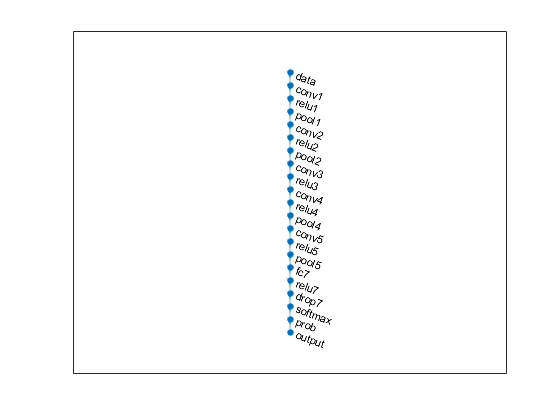
\includegraphics[scale=0.5]{figure_13.png}
\end{center}


\label{H_01F04CB8}
\matlabheading{4.2 Learning Curves and Training Process}

\begin{par}
\begin{flushleft}
We trained the network on single GPU system nad print the results in a table every 50 iterations. Besides, the learning curves are plotted after the table. Finally the network reached 85.16\% on training and 81.56\% on validation subset. The training process took about 88 minutes long.
\end{flushleft}
\end{par}

\begin{matlabcode}
trained_net_4 = trainNetwork(augimdsTrain, layers_4, opts);
\end{matlabcode}
\begin{matlaboutput}
Training on single GPU.
Initializing input data normalization.
|===============================================================================================================|
|  Epoch  |  Iteration  |  Time Elapsed  |  Mini-batch  |  Validation  |  Mini-batch  |  Validation  |  Base Learning  |
|         |             |   (hh:mm:ss)   |   Accuracy   |   Accuracy   |     Loss     |     Loss     |      Rate       |
|===============================================================================================================|
|       1 |           1 |       00:00:09 |       11.72% |       10.12% |      10.5038 |       9.4881 |          0.0010 |
|       1 |          50 |       00:01:26 |       23.83% |       32.83% |       2.1314 |       1.8730 |          0.0010 |
|       2 |         100 |       00:02:44 |       38.28% |       42.65% |       1.7415 |       1.5924 |          0.0010 |
|       2 |         150 |       00:04:03 |       43.16% |       45.68% |       1.6198 |       1.4808 |          0.0010 |
|       3 |         200 |       00:05:23 |       43.95% |       51.21% |       1.5060 |       1.3415 |          0.0010 |
|       4 |         250 |       00:06:44 |       50.39% |       53.56% |       1.3679 |       1.3049 |          0.0010 |
|       4 |         300 |       00:08:03 |       53.32% |       55.84% |       1.3522 |       1.2311 |          0.0010 |
|       5 |         350 |       00:09:23 |       56.64% |       59.04% |       1.2368 |       1.1214 |          0.0010 |
|       5 |         400 |       00:10:42 |       55.86% |       60.37% |       1.2420 |       1.0968 |          0.0010 |
|       6 |         450 |       00:12:02 |       64.65% |       62.09% |       1.0527 |       1.0670 |          0.0010 |
|       7 |         500 |       00:13:21 |       65.63% |       63.21% |       1.0031 |       1.0294 |          0.0010 |
|       7 |         550 |       00:14:40 |       64.45% |       66.41% |       1.0214 |       0.9567 |          0.0010 |
|       8 |         600 |       00:15:59 |       66.80% |       66.57% |       0.9318 |       0.9426 |          0.0010 |
|       8 |         650 |       00:17:17 |       66.41% |       69.12% |       0.9867 |       0.8769 |          0.0010 |
|       9 |         700 |       00:18:36 |       71.29% |       71.09% |       0.8586 |       0.8371 |          0.0010 |
|      10 |         750 |       00:19:55 |       70.12% |       68.80% |       0.8572 |       0.8933 |          0.0010 |
|      10 |         800 |       00:21:13 |       69.53% |       70.80% |       0.8742 |       0.8329 |          0.0010 |
|      11 |         850 |       00:22:32 |       70.90% |       72.91% |       0.8471 |       0.7851 |          0.0010 |
|      11 |         900 |       00:23:50 |       74.22% |       72.27% |       0.7121 |       0.7916 |          0.0010 |
|      12 |         950 |       00:25:09 |       73.24% |       71.33% |       0.7878 |       0.8584 |          0.0010 |
|      13 |        1000 |       00:26:27 |       77.93% |       72.17% |       0.6161 |       0.8177 |          0.0010 |
|      13 |        1050 |       00:27:46 |       75.00% |       74.36% |       0.7175 |       0.7403 |          0.0010 |
|      14 |        1100 |       00:29:04 |       76.17% |       73.64% |       0.7260 |       0.7520 |          0.0010 |
|      14 |        1150 |       00:30:22 |       76.76% |       75.37% |       0.6979 |       0.7155 |          0.0010 |
|      15 |        1200 |       00:31:40 |       76.17% |       75.59% |       0.6442 |       0.7154 |          0.0010 |
|      16 |        1250 |       00:32:59 |       76.95% |       75.53% |       0.6579 |       0.7148 |          0.0010 |
|      16 |        1300 |       00:34:17 |       75.78% |       76.36% |       0.7088 |       0.7086 |          0.0010 |
|      17 |        1350 |       00:35:35 |       79.49% |       75.55% |       0.6131 |       0.7544 |          0.0010 |
|      17 |        1400 |       00:36:53 |       75.78% |       74.63% |       0.6773 |       0.7344 |          0.0010 |
|      18 |        1450 |       00:38:11 |       80.08% |       77.29% |       0.6093 |       0.6770 |          0.0010 |
|      19 |        1500 |       00:39:29 |       80.66% |       76.27% |       0.5871 |       0.6974 |          0.0010 |
|      19 |        1550 |       00:40:47 |       77.15% |       77.79% |       0.6782 |       0.6573 |          0.0010 |
|      20 |        1600 |       00:42:05 |       79.10% |       78.64% |       0.6255 |       0.6601 |          0.0010 |
|      20 |        1650 |       00:43:23 |       81.25% |       77.33% |       0.6001 |       0.6815 |          0.0010 |
|      21 |        1700 |       00:44:42 |       77.93% |       76.87% |       0.6048 |       0.6655 |          0.0010 |
|      22 |        1750 |       00:46:00 |       82.81% |       78.67% |       0.4991 |       0.6453 |          0.0010 |
|      22 |        1800 |       00:47:25 |       77.73% |       78.15% |       0.6271 |       0.6564 |          0.0010 |
|      23 |        1850 |       00:48:44 |       76.76% |       77.64% |       0.6390 |       0.6833 |          0.0010 |
|      23 |        1900 |       00:50:03 |       82.42% |       78.17% |       0.5483 |       0.6655 |          0.0010 |
|      24 |        1950 |       00:51:23 |       79.88% |       77.65% |       0.5369 |       0.6748 |          0.0010 |
|      25 |        2000 |       00:52:43 |       82.42% |       78.63% |       0.5254 |       0.6525 |          0.0010 |
|      25 |        2050 |       00:54:03 |       83.98% |       79.60% |       0.4554 |       0.6171 |          0.0010 |
|      26 |        2100 |       00:55:22 |       83.59% |       79.52% |       0.4978 |       0.6169 |          0.0010 |
|      26 |        2150 |       00:56:41 |       83.20% |       78.80% |       0.4724 |       0.6680 |          0.0010 |
|      27 |        2200 |       00:57:59 |       82.81% |       80.08% |       0.5037 |       0.6214 |          0.0010 |
|      28 |        2250 |       00:59:18 |       86.52% |       80.93% |       0.3928 |       0.6083 |          0.0010 |
|      28 |        2300 |       01:00:37 |       86.13% |       79.84% |       0.4347 |       0.5991 |          0.0010 |
|      29 |        2350 |       01:01:56 |       79.88% |       80.29% |       0.5154 |       0.6146 |          0.0010 |
|      29 |        2400 |       01:03:14 |       83.20% |       80.00% |       0.5069 |       0.6028 |          0.0010 |
|      30 |        2450 |       01:04:34 |       85.16% |       78.81% |       0.4108 |       0.6991 |          0.0010 |
|      31 |        2500 |       01:05:53 |       83.01% |       80.20% |       0.4772 |       0.5975 |          0.0010 |
|      31 |        2550 |       01:07:12 |       81.05% |       79.15% |       0.5888 |       0.6645 |          0.0010 |
|      32 |        2600 |       01:08:31 |       84.57% |       79.93% |       0.4370 |       0.6453 |          0.0010 |
|      32 |        2650 |       01:09:49 |       85.94% |       80.13% |       0.4144 |       0.6194 |          0.0010 |
|      33 |        2700 |       01:11:08 |       85.55% |       78.76% |       0.4232 |       0.6549 |          0.0010 |
|      34 |        2750 |       01:12:26 |       83.79% |       81.27% |       0.4577 |       0.5956 |          0.0010 |
|      34 |        2800 |       01:13:45 |       84.57% |       79.92% |       0.4605 |       0.6482 |          0.0010 |
|      35 |        2850 |       01:15:04 |       85.16% |       80.64% |       0.4686 |       0.6112 |          0.0010 |
|      35 |        2900 |       01:16:23 |       85.35% |       80.91% |       0.4015 |       0.5787 |          0.0010 |
|      36 |        2950 |       01:17:42 |       84.77% |       80.65% |       0.4368 |       0.6163 |          0.0010 |
|      37 |        3000 |       01:19:01 |       86.52% |       81.67% |       0.3710 |       0.6021 |          0.0010 |
|      37 |        3050 |       01:20:19 |       84.38% |       82.09% |       0.4289 |       0.5681 |          0.0010 |
|      38 |        3100 |       01:21:38 |       87.11% |       81.64% |       0.3445 |       0.5873 |          0.0010 |
|      38 |        3150 |       01:22:57 |       85.55% |       81.47% |       0.4172 |       0.5899 |          0.0010 |
|      39 |        3200 |       01:24:15 |       86.13% |       81.55% |       0.4324 |       0.5927 |          0.0010 |
|      40 |        3250 |       01:25:35 |       86.13% |       81.41% |       0.4079 |       0.6028 |          0.0010 |
|      40 |        3300 |       01:26:53 |       84.96% |       80.73% |       0.4284 |       0.6104 |          0.0010 |
|      40 |        3320 |       01:27:29 |       85.16% |       81.56% |       0.4182 |       0.6244 |          0.0010 |
|===============================================================================================================|
\end{matlaboutput}
\begin{center}
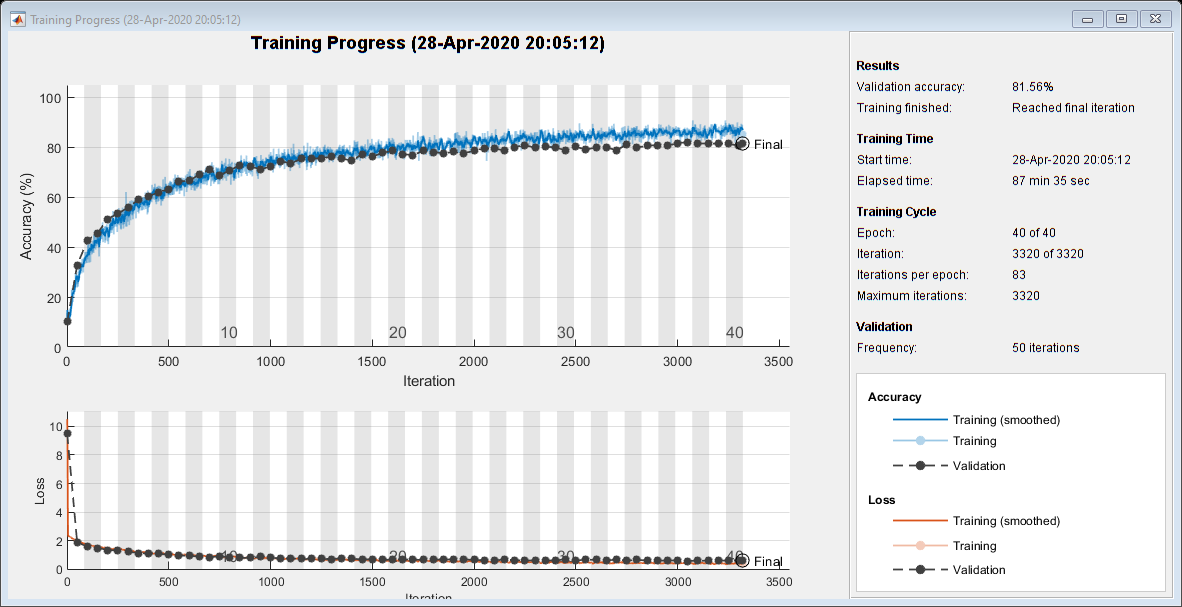
\includegraphics[width=\maxwidth{80.28098344204717em}]{figure_14.png}
\end{center}


\label{H_4D1F1553}
\matlabheading{4.3 Evaluating the Network}

\begin{par}
\begin{flushleft}
Here we use the test partition of the dataset to evaluate the trained network.
\end{flushleft}
\end{par}

\label{H_8964CC3C}
\matlabheadingtwo{4.3.1 Classifying the Test Dataset}

\begin{par}
\begin{flushleft}
The line below will classify all images in the test dataset.
\end{flushleft}
\end{par}

\begin{matlabcode}
predicted_labels_4 = classify(trained_net_4, imds_test);
\end{matlabcode}


\label{H_DCC7C50E}
\matlabheadingtwo{4.3.2 Classification Performance}

\begin{par}
\begin{flushleft}
As the final step of this section, we plot the confusion matrix. The final performance of the network is 81.2\% over the whole test dataset.
\end{flushleft}
\end{par}

\begin{matlabcode}
plotconfusion(imds_test.Labels, predicted_labels_4);
\end{matlabcode}
\begin{center}
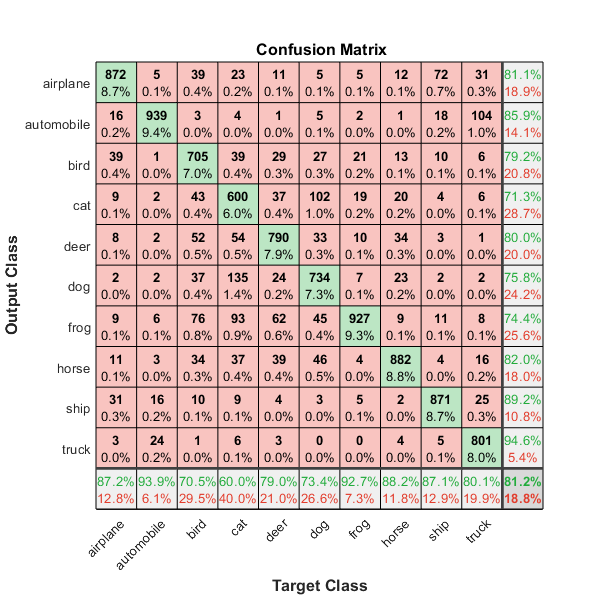
\includegraphics[scale=0.6]{figure_15.png}
\end{center}

\clearpage
\label{T_0A1F9F85}
\matlabtitle{Appendix}

\label{H_412958D7}
\matlabheading{A.1 Saving Workspace Variables for Future Use }

\begin{matlabcode}
save('HW8_code_workspace.mat')
\end{matlabcode}
\label{H_031328DF}
\matlabheading{A.2 Definition of Auxiliary Functions}
\begin{matlabcode}
function saveCIFAR10AsFolderOfImages(inputPath, outputPath, varargin)

% Check input directories are valid
if(~isempty(inputPath))
    assert(exist(inputPath,'dir') == 7);
end
if(~isempty(outputPath))
    assert(exist(outputPath,'dir') == 7);
end

% Check if we want to save each set with the same labels to its own
% directory.
if(isempty(varargin))
    labelDirectories = false;
else
    assert(nargin == 3);
    labelDirectories = varargin{1};
end

% Set names for directories
trainDirectoryName = 'cifar10Train';
testDirectoryName = 'cifar10Test';
% Create directories for the output
mkdir(fullfile(outputPath, trainDirectoryName));
mkdir(fullfile(outputPath, testDirectoryName));

if(labelDirectories)
    labelNames = {'airplane','automobile','bird','cat','deer','dog','frog','horse','ship','truck'};
    iMakeTheseDirectories(fullfile(outputPath, trainDirectoryName), labelNames);
    iMakeTheseDirectories(fullfile(outputPath, testDirectoryName), labelNames);
    for i = 1:5
        iLoadBatchAndWriteAsImagesToLabelFolders(fullfile(inputPath,['data_batch_' num2str(i) '.mat']), fullfile(outputPath, trainDirectoryName), labelNames, (i-1)*10000);
    end
    iLoadBatchAndWriteAsImagesToLabelFolders(fullfile(inputPath,'test_batch.mat'), fullfile(outputPath, testDirectoryName), labelNames, 0);
else
    for i = 1:5
        iLoadBatchAndWriteAsImages(fullfile(inputPath,['data_batch_' num2str(i) '.mat']), fullfile(outputPath, trainDirectoryName), (i-1)*10000);
    end
    iLoadBatchAndWriteAsImages(fullfile(inputPath,'test_batch.mat'), fullfile(outputPath, testDirectoryName), 0);
end
end

function iLoadBatchAndWriteAsImagesToLabelFolders(fullInputBatchPath, fullOutputDirectoryPath, labelNames, nameIndexOffset)
load(fullInputBatchPath);
data = data'; %#ok<NODEF>
data = reshape(data, 32,32,3,[]);
data = permute(data, [2 1 3 4]);
for i = 1:size(data,4)
    imwrite(data(:,:,:,i), fullfile(fullOutputDirectoryPath, labelNames{labels(i)+1}, ['image' num2str(i + nameIndexOffset) '.png']));
end
end

function iLoadBatchAndWriteAsImages(fullInputBatchPath, fullOutputDirectoryPath, nameIndexOffset)
load(fullInputBatchPath);
data = data'; %#ok<NODEF>
data = reshape(data, 32,32,3,[]);
data = permute(data, [2 1 3 4]);
for i = 1:size(data,4)
    imwrite(data(:,:,:,i), fullfile(fullOutputDirectoryPath, ['image' num2str(i + nameIndexOffset) '.png']));
end
end

function iMakeTheseDirectories(outputPath, directoryNames)
for i = 1:numel(directoryNames)
    mkdir(fullfile(outputPath, directoryNames{i}));
end
end

function h = subplottight(n,m,i)
[c,r] = ind2sub([m n], i);
ax = subplot('Position', [(c-1)/m, 1-(r)/n, 1/m, 1/n]);
if(nargout > 0)
  h = ax;
end
end
\end{matlabcode}

\end{document}
